\section{Datenmodell}
\setauthor{Hain Lukas}

\begin{figure}[H]
    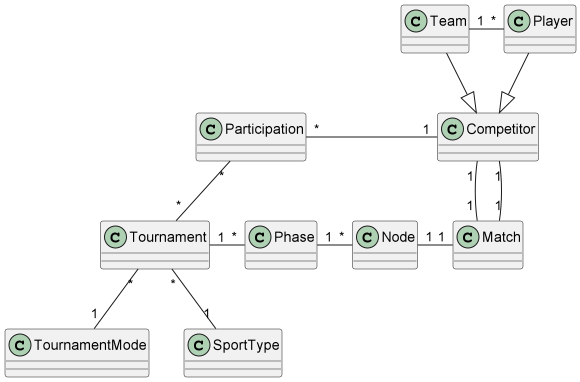
\includegraphics[scale=1]{pics/backend/class_diagram.png}
    \caption{Class Diagram}
\end{figure}

Oben abgebildet ist das Datenmodell des Quarkus Backends. Anfangs erstellt man ein Turnier (Tournament), neben Namen, Startdatum und Enddatum 
wird hier noch der Turniermodus (TournamentMode) und die Sportart (SportType) festgelegt. Nun gibt man an, welche Teilnehmer/innen (Competitor) an diesem Turnier teilnehmen (Participation). 
Ein Competitor kann entweder ein einzelner Spieler (Player) oder ein Team von Spielern (Team) sein.
Wenn das Turnier gestartet wird, wird das Turnier in Phasen (Phase) unterteilt. In jeder Phase gibt es eine bestimmte Anzahl an Matches (Match), welche jeweils 2 Competitor haben und mithilfe von Nodes (Node) 
der jeweiligen Phase zugeordnet werden.

\section{Quarkus Backend}
\setauthor{Hain Lukas}

\subsection{Ordnerstruktur}

\begin{figure}[H]
    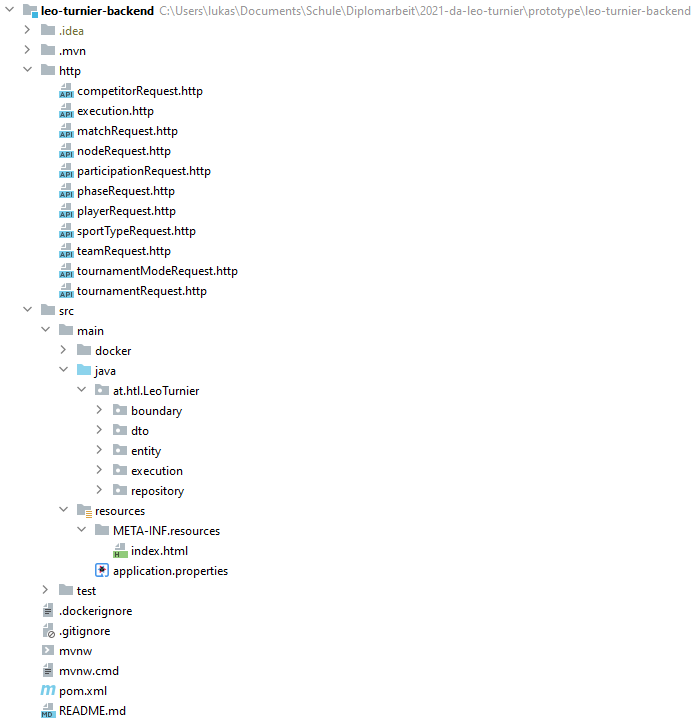
\includegraphics[scale=0.8]{pics/backend/quarkus_file_structure.png}
    \caption{Quarkus Ordnerstruktur}
\end{figure}

Nach dem erstellen eines Quarkus Projektes ist ein Großteil der Ordnerstruktur bereits im vorhinein gegeben. Das wichtigste File im Projekt befindet sich ganz im äußersten Ordner, nämlich das "pom.xml" File. 

\begin{figure}[H]
    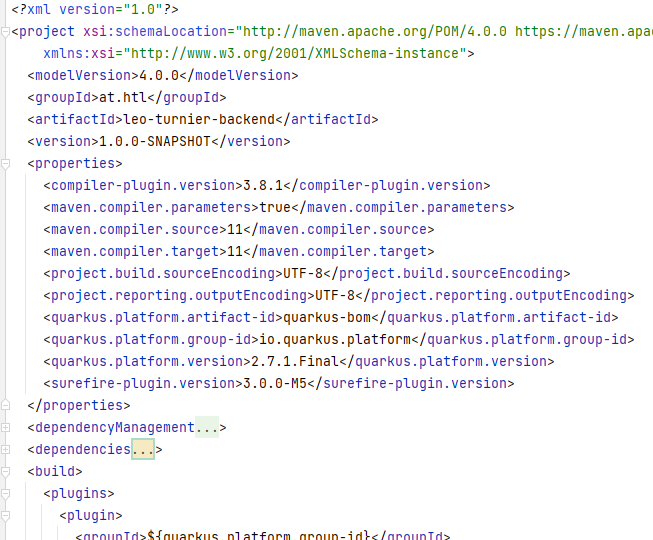
\includegraphics[scale=0.6]{pics/backend/pom.xml.png}
    \caption{pom.xml}
\end{figure}

Hier werden nicht nur die Metadaten des Projekts angegeben, sondern auch die Dependencies, also alle externen Libraries, die die Applikation benötigt. 

Im "src" Ordner befinden sich ein "main" und ein "test" Ordner. Im "main" Ordner befindet sich der ganze Quellcode der Applikation, und im "test" Ordner befindet sich der Code, der den Quellcode auf seine richtigkeit prüft.
Im "main" Ordner befindet sich nun ein "docker" Ordner, auf den später noch eingegangen wird, ein "java" Ordner, in dem sich die Java Klassen der Applikation befindet, und ein "resources" Ordner, in dem weitere Files zu finden sind, 
auf die der Java Code eventuell zugreifen kann. Außerdem befindet sich im "resources" Ordner das "application.properties" File, in dem verschiedene Quarkus Konfigurationen zu finden sind.

\begin{figure}[H]
    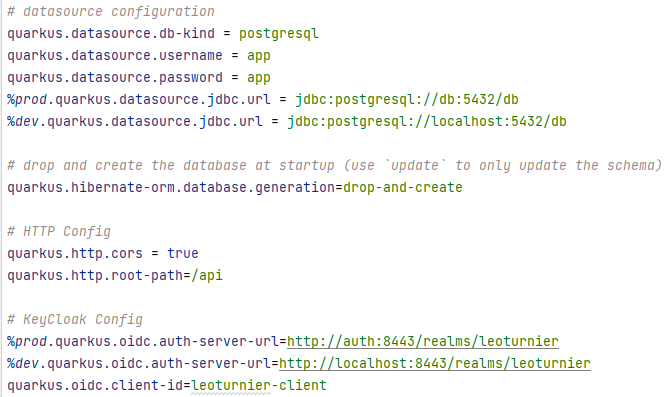
\includegraphics[scale=0.6]{pics/backend/application.properties.png}
    \caption{application.properties}
\end{figure}

Die Konfigurationen sind aufgeteilt in Datasource (Datenbank), HTTP (Endpoints) und KeyCloak Konfigurationen. 

(Ist der Teil unten zu Basic?) (Der Teil unten gehört noch zur "Quarkus Ordnerstruktur" Abbildung, kann sein dass das etwas unklar ist, wie könnte ich das am besten machen?)

Die Java Klassen im "java" Ordner sind weiters in 5 verschiedene Ordner aufgeteilt. Im "entity" Ordner befinden sich alle Entitätsklassen der Applikation, also jene, die das Datenmodell (siehe Kapitel 6.1 Datenmodell) wiederspiegeln.
Die Klassen im "repository" sind die Schnittstelle zwischen der Quarkus Applikation und der Datenbank. Sie sind für die CRUD Operationen verantwortlich, also das Speichern, Auslesen, Verändern oder Löschen von Daten nach dem Schema der Entitätsklassen.
Außerdem befindet sich hier die Logik hinter den Turnieren. Die Klassen im "boundary" sind die Schnittstelle zum Frontend. Sie nehmen Requests, also Anforderungen, von außen an, 
führen die jeweilige Methode aus den Repository Klassen aus und liefern dann eine Response, also eine Antwort, zurück. Als nächstes gibt es die im "execution" Ordner, diese sind für die Durchführung der Turniere zuständig, hier befindet sich auch der Großteil der Logik. 
Zuletzt gibt es noch die Klassen in "dto" Ordner, diese sind Klassen, in denen Daten gespeichert werden können, die für die Logik in den Repository Klassen benötigt wird, jedoch nicht unbedingt Teil des Datenmodells sind.

\subsection{Entitätsklassen}

\begin{figure}[H]
    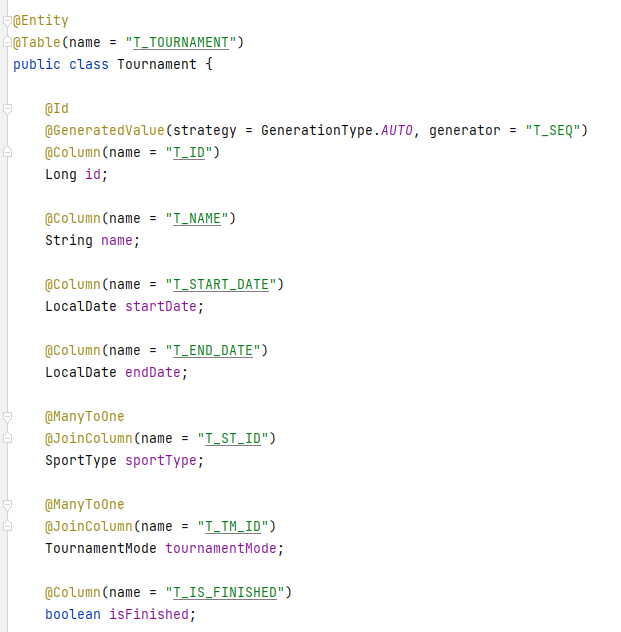
\includegraphics[scale=0.8]{pics/backend/entity_class.png}
    \caption{Entitätsklasse}
\end{figure}

Oben abgebildet ist eine der Entitätsklassen dieser Applikation, nämlich die Tournament Klasse. Ganz oben, über der Klasse, ist die Annotation "@Entity" zu finden, um sicherzustellen, dass die Klasse von JPA als Entitätsklasse erkannt wird, 
und das Library dafür eine Tabelle erstellt. Darunter befindet sich die "@Table" Annotation, die der Tabelle in der Datenbank ihren Namen gibt. Das Schema der Namensgebung von Tabellen lautet wie folgt: 
am Anfang steht immer die Abkürzung für den Tabellennamen, in diesem Fall ist das "T", danach kommt ein Unterstrich, gefolgt von dem Namen der Entitätsklasse in Großbuchstaben. 
In der Klasse selbst befinden sich nun die Klassenvariablen, welche von der Annotation "@Column" ihren Namen in der Datenbank verleiht. Das Schema der Namensgebung ist ähnlich, wie das der Tabellen: 
Anfangs die Abkürzung des Tabellennamens, dann ein Unterstrich als Trennung, gefolgt vom Namen der Klassenvariable, ebenfalls in Großbuchstaben. Die ID hat eine extra annotation, nämlich "@Id", 
das bedeutet dass sie der Primärschlüssel der Entitätsklasse ist. Wie der Wert der Id generiert wird, wird mit "@GeneratedValue" festgelegt. Außerdem steht bei den Variablen "tournamentmode" und "sportType" noch die "@ManyToOne" Annotation. 
Diese Felder werden dann in der Datenbank zu den Fremdschlüsseln auf andere Tabellen. Hier lautet das Namensschema wie folgt: Zuerst die Abkürzung der eigenen Klasse, 
dann der Name des Primärschlussels aus der Tabelle, auf die der Fremdschlüssel zeigt, wieder, getrennt durch einen Unterstrich.
Es gibt 4 Verschiedene Annotationen, die eine Beziehung zu anderen Tabellen herstellen:

\begin{itemize}
    \item @OneToOne
    \item @ManyToOne
    \item @OneToMany
    \item @ManyToMany
\end{itemize}

(wie könnte ich unten noch zu der "anderen" Klasse sagen?)

Die erste Mengenangabe steht immer für die eigene Klasse, die zweite steht für die andere Klasse. Diese braucht in diesem Fall natürlich auch die "@Entity" Annotation sowie einen Primärschlüssel. 
Bei "@OneToOne" und "@ManyToOne" wird in der Datenbank der Fremdschlüssel in der eigenen Tabelle erstellt, bei "@OneToMany" wird der Fremdschlüssel in der anderen Tabelle 
erstellt (hier muss die Variable, bei der die Annotation steht, auch eine Collection sein), und bei "@ManyToMany" wird eine Assotiationstabelle erstellt, in der sich dann 2 Fremdschlüssel befinden: 
einmal der au die Tabelle der eigenen Klasse, und einmal die der naderen Klasse.

Unter den Klassen befinden sich dann standardmäßig noch der Constructor sowie die Getter und Setter.

\subsection{Repositoryklassen}

\begin{figure}[H]
    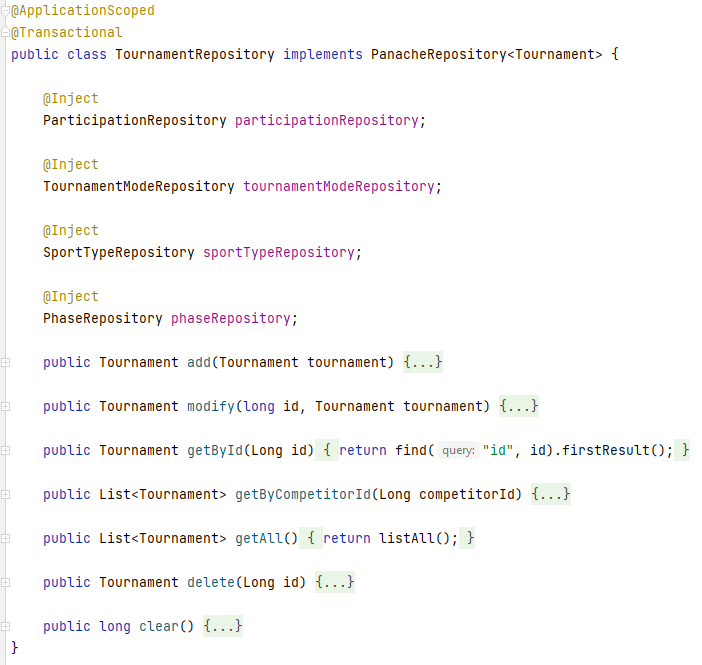
\includegraphics[scale=0.8]{pics/backend/repository_class.png}
    \caption{Repositoryklasse}
\end{figure}

Wie oben schon erwähnt sind die Repositoryklassen die Schnittstelle zwischen Quarkus Backend und Datenbank, dies wird durch die "Hibernate ORM with Panache" Library ermöglicht. 
Außer ein paar Ausnahmen befinden sich hier nur die CRUD (Create - Read - Update - Delete) Operationen, als Create Operation fungiert hier die "add" Methode, 
als Read Operationen die "get" Methoden (getById, getByCompetitorId, getAll), als Update Operation die "modify" Methode und als Delete Operationen die "delete" und "clear". 
Über der Klasse befinden sich die Annotation "@ApplicationScoped" und "@Transactional". "@ApplicationScoped" ermöglicht es anderen Repositoryklassen, mithilfe von "@Inject" eine Instanz dieser Klasse zu injezieren, genau so, 
wie es diese Klasse weiter unten auch tut. Es wird zum Beispiel in der "add" Methode "TournamentRepository" Klasse (siehe Abbildung "add Methode aus TournamentRepository" unten) die 
der "SportTypeRepository" Klasse benötigt, da sich in der "Tournament" Klasse ein Fremdschlüssel auf die "SportType" Klasse befindet. Sollte also die Sportart, 
auf die dieser Fremdschlüssel zeigt, in der Datenbank nicht existieren, kommt es zu einer SQLException, wesshalb in der add Mehode von "TournamentRepository", 
bevor das Turnier selbst mit "persist" gespeichert wird, nocht die Sportart mithilfe der add Methode der "SportTypeRepository" Klasse in der Datenbank. 

\begin{figure}[H]
    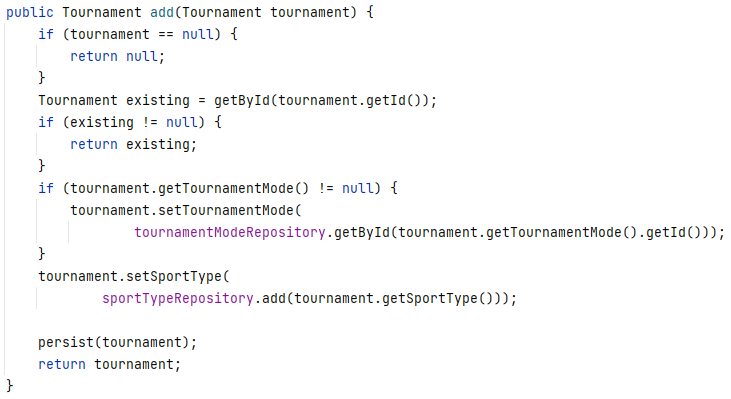
\includegraphics[scale=0.8]{pics/backend/repository_add_function.png}
    \caption{add Methode aus TournamentRepository}
\end{figure}

Das gleiche passiert bei der "modify" Methode, wenn der Fremdschlüssel auf eine Sportart zeigt, die noch nicht existiert.

"@Transactional" wird verwendet, um in jeder Methode dieser Klasse vor den Ausführen eine neue Transaktion zu erstellen, und diese danach zu commiten. 
Wenn Daten in der Datenbank gespeichert, modifiziert oder gelöscht werden, werden diese Änderungen erst dann wirklich in die Datenbank übernommen, wenn eine Transaktion commitet wurde.

Das PanacheRepository ist eine Erweiterung aus dem "Hibernate ORM \textbf{with Panache}" Library, ohne Panache wäre theoretisch auch alles, was in den Repositoryklassen Implementiert wurde, möglich, jedoch etwas umständlicher.
Zum Beispiel gibt es ohne Panache die "persist" Methode nicht, in dem Fall müsste man eine "EntityManager" Instanz mithilfe von Dependency Injection injezieren, in davon dann die "persist" Methode hernehmen.
Auch andere Methoden, wie zum Beispiel "find" oder "listAll" wären ohne Panach nicht verfügbar, und müssten vom Entwickler selbst Implementiert werden.

\subsection{Serviceklassen}

\begin{figure}[H]
    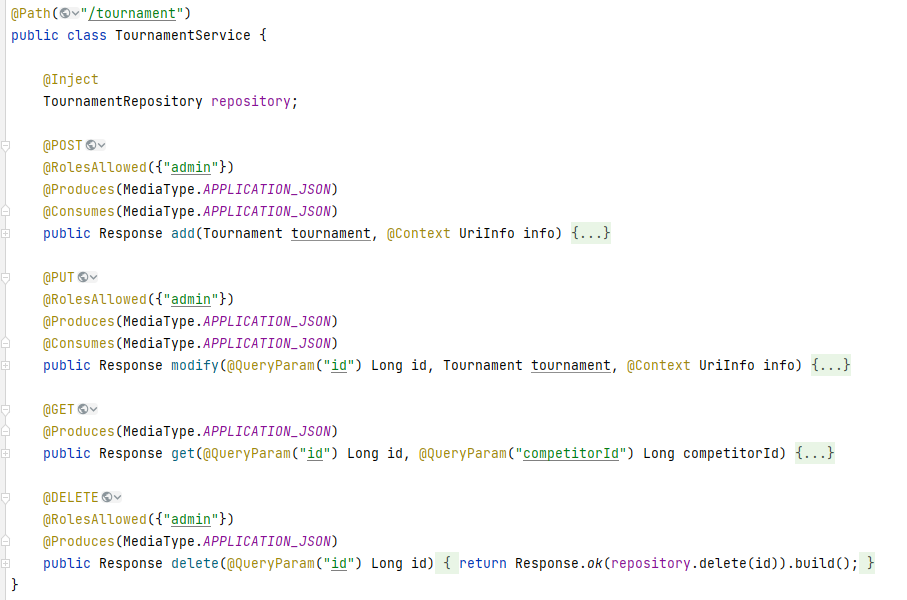
\includegraphics[scale=0.6]{pics/backend/service_class.png}
    \caption{Serviceklasse}
\end{figure}

Die Serviceklassen sind die Schnittstelle zum Frontend, diesem stellen sie durch Endpoints, welche von Requests angesprochen werden, Daten aus der Datenbank zur Verfügung, dies wird durch die "RESTEasy" Library ermöglicht.
Über der Klasse wird mithilfe der Annotation "@Path" der URL Path zu den Endpoints dieser Klasse festgestellt. In der Klasse selbst wird zuerst eine Instanz des dazugehörigen Repositories injeziert. 
Danach folgt für jede CRUD Operation ein Endpoint. Es gibt verschiedene Arten von Endpoints, in dieser Applikation werden hauptsächlich 4 verwendet:

\begin{itemize}
    \item "@POST" bei Create Operationen
    \item "@PUT" bei Update Operationen
    \item "@GET" bei Read Operationen
    \item "@DELETE" bei Delete Operationen
\end{itemize}

"@RolesAllowed" gibt an, welche Rollen zugriff auf diesen Enpoint haben. Darauf wird im Kapitel KeyCloak noch genauer eingegangen. "@Consumes" und "@Produces" geben an, 
welche Art von Content in den Requests (@Consumes) bzw. den Responses (@Produces) übergeben werden soll. Außerdem wäre es noch möglich, den URL Path zu einem bestimmten Endpoint zu ändern, 
und zwar wieder mit der "@Path" Annotation. Bei den Parametern der Methoden gibt es manche mit der Annotation "@QueryParam", diese Annotation gibt an, dass dieser Parameter von der 
Request in der URL definiert wird. Zum Beispiel sieht die URL einer Request auf den GET Endpoint wie folgt aus:

\textbf{http://localhost:8080/api/tournament?id=1} 

Der Hostname ist in diesem Quarkus Backend "localhost", der Port 8080, der Root Path "api" wurde im "application.properties" File festgelegt, und der Path "tournament" wie erwähnt mit der "@Path" Annotation. 
Nach dem "?" werden immer die Queryparameter ("@QueryParam") übergeben, in diesem Fall die "id" mit dem Wert 1. Der Parameter "UriInfo" wird benötigt, um im Header der Response den Path zurückzugeben, 
mit dem man den neu hinzugefügten bzw. modifizierten Datensatz finden kann.

Was bei den Serviceklassen noch auffallend ist, ist dass es zum Beispiel für Read Operationen insgesammt nur einen Endpoint pro Serviceklasse gibt, obwohl es in den Repositoryklassen mehrere Get Methoden gibt (siehe Abbildung "Repositoryklasse").
Dies wird dadurch gelöst, dass Endpoints auch erfolgreich ausgeführt werden, wenn nicht alle Queryparameter in der URL definiert wurden, diese haben standardmäßig den Wert "null". Mit diesem Prinzib wird erreicht, dass mit dem gleichen URL Path 
verschiedene Read Operationen durchführen kann.

\begin{figure}[H]
    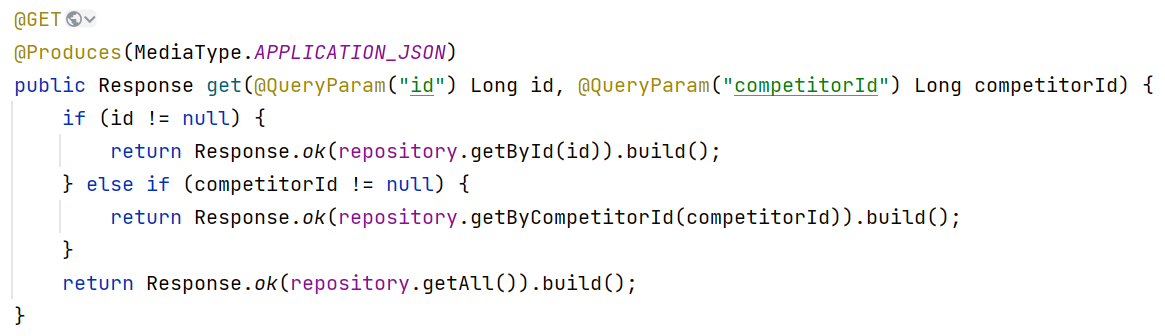
\includegraphics[scale=0.5]{pics/backend/service_get_function.png}
    \caption{get Methode aus TournamentService}
\end{figure}

Im obigen Beispiel hat man 3 Möglichkeiten:

\begin{itemize}
    \item keinen Query Parameter anzugeben, um alle Turniere auszulesen
    \item den "id" Query Parameter anzugeben, um nur das Turnier mit der angegebenen Id auszulesen
    \item den "competitorId" Query Parameter anzugeben, um alle Turniere auszulesen, in denen der Competitor mit der angegebenen Id dabei war.
\end{itemize}

Die einzige Entitätsklasse, für die es nur READ Endpoints gibt, ist die TournamentMode Klasse, Turniermodi werden beim Start des Backends mithilfe der "InitBean" Klasse 
automatisch in die Datenbank hinzugefügten, da diese für die Turnierdurchführung jeweils einzeln Implementiert werden müssen.

\subsection{Turnierdurchführung}

Für die Turnierdurchführung gibt es insgesammt 4 verschiedene Durchführungsklassen, eine für jeden Turniermodus (Elimination, Round Robin, Combination), und eine als Schnittstelle zu den Serviceklassen, welche aus den anderen 3 
die richtigen Methoden ausführen soll, abhängig davon, welchen Turniermodus das Turnier hat. 

\begin{figure}[H]
    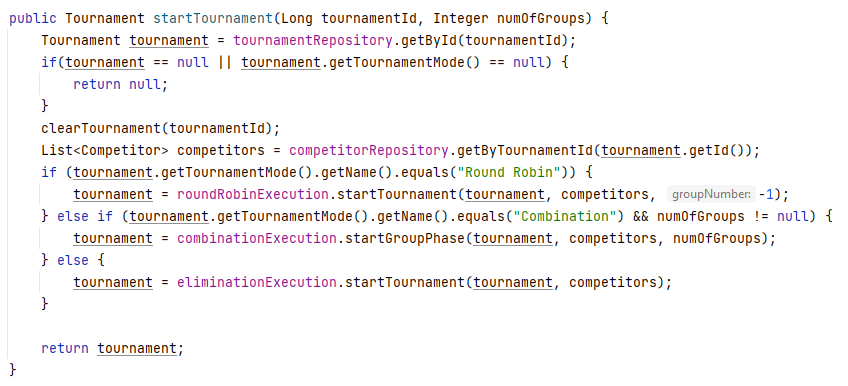
\includegraphics[scale=0.65]{pics/backend/execution_startTournament.png}
    \caption{"startTournament" Methode der Execution Klasse}
\end{figure}

In der "startTournament" Methode zum Beispiel wird, nachdem alle vorherigen Matches usw. daraus gelöscht wurden, die "startTournament" Methode aus der dem TurnierModus entsprechenden Durchführungsklasse ausgeführt, 
bzw. im Falle des "Combination" Turniermodus die "startGroupPhase" Methode (mehr dazu weiter unten).

\subsection{Elimination}

Im Elimination Turniermodus scheidet nach einem Match der Verlierer sofort aus dem Turnier aus, und der Gewinner steigt in die nächste Runde auf. 
Das Ganze wiederholt sich so lange, bis nur noch ein/eine Teilnehmer/in übrig bleibt, dieser ist dann der Sieger des Turniers. So entsteht dann der klassische Turnierbaum.

\begin{figure}[H]
    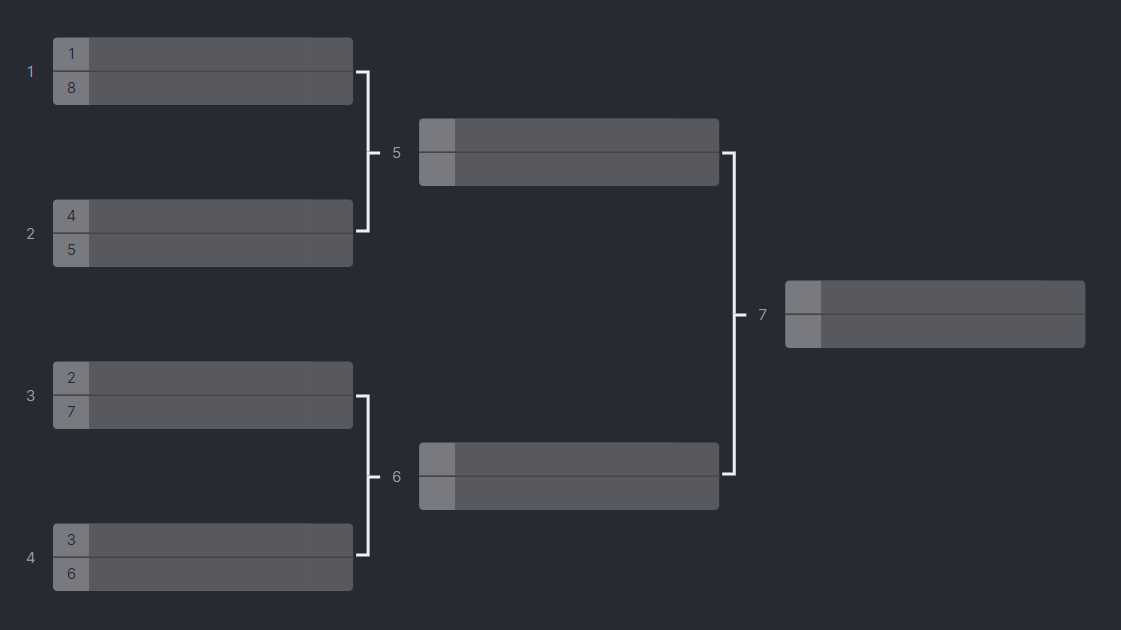
\includegraphics[scale=0.5]{pics/backend/elimination/elimination_tree.png}
    \caption{Turnierbaum\cite{implementation-execution-1}}
\end{figure}

\subsubsection{Phases}

Ein Turnier ist in Phasen aufgeteilt, in der Abbildung oben ist jede Spalte von Matches eine Phase. Die Phasen eines Turniers werden mit der folgenden Methode eingefügt.

\begin{figure}[H]
    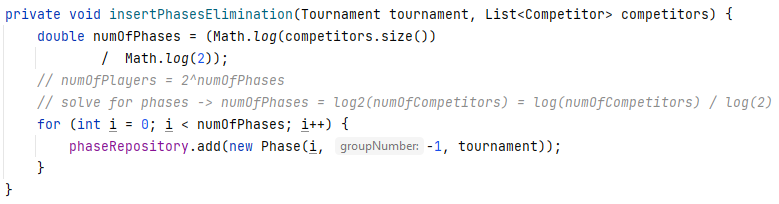
\includegraphics[scale=0.7]{pics/backend/elimination/elimination_insertPhases.png}
    \caption{Einfügen der Phasen im Elimination Modus}
\end{figure}

Zuerst wird die Anzahl der Phasen anhand der Teilnehmeranzahl berechnet. Dies erfolgt mit dem Logarithmus zur Basis 2 von der Teilnehmeranzahl (log\textsubscript{2}(n)). 
Da es in Java nicht möglich ist, die Basis eines Logarithmus frei zu wählen, wird stattdessen der Logarithmus der Teilnehmeranzahl dividiert durch den 
Logarithmus der Basis gerechnet, was zum gleichen Ergebnis kommt (log(n)/log(2)). Anschließend werden die Phasen numeriert in die Datenbank gespeichert, von 0 beginnend.

\subsubsection{Nodes}

Als nächstes werden zu jeder Phase Nodes eingefügt, diese bilden zusammen mit den Phasen das Grundgerüst des Turniers. 

\begin{figure}[H]
    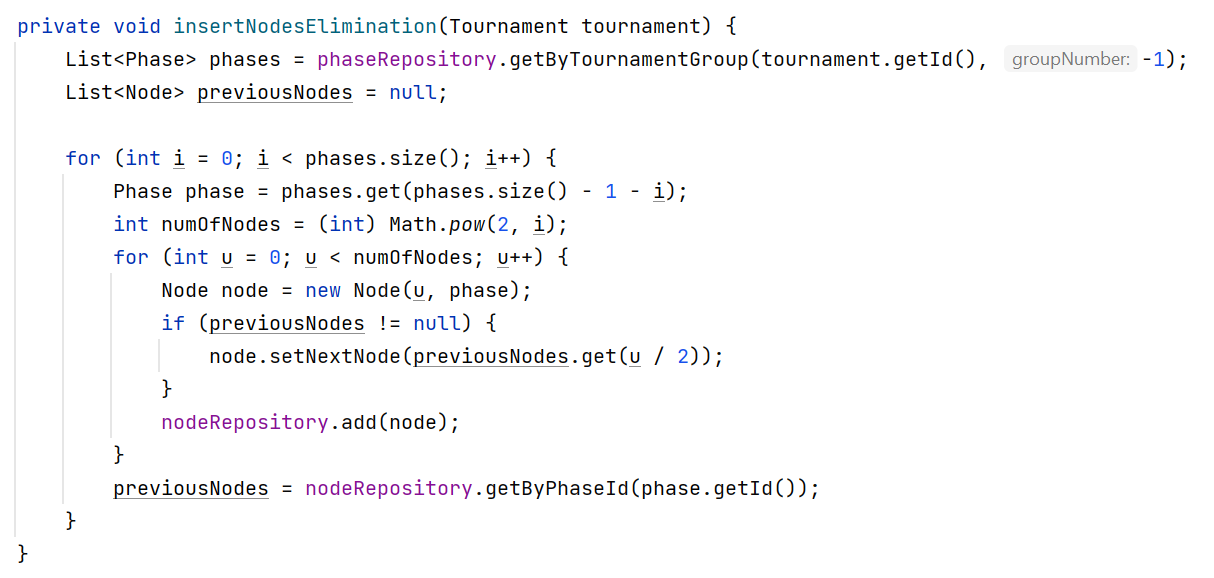
\includegraphics[scale=0.48]{pics/backend/elimination/elimination_insertNodes.png}
    \caption{Einfügen der Nodes im Elimination Modus}
\end{figure}

Es wird rückwärts durch die Phasen des Turniers iteriert, sodass, die letzte Phase am Ende nur einen Node hat, nämlich das Finale.
Anschließend wird die Anzahl an Nodes für die momentane Phase berechnet, dies erfolgt mit der Rechnung 2 Hoch die Teilnehmeranzahl (2\textsuperscript{n}). 
Anschließend wird für jeden Node der "nextNode" gesetzt, das ist jener Node, in den der Sieger des Matches aus dem momentanen Nodes aufsteigen würde, 
und diese dann in die Datenbank eingefügt.

\subsubsection{Matches}

Zu jedem Node im Turnierbaum gehört ein Match, diese werden mit der folgenden Methode eingefügt.

\begin{figure}[H]
    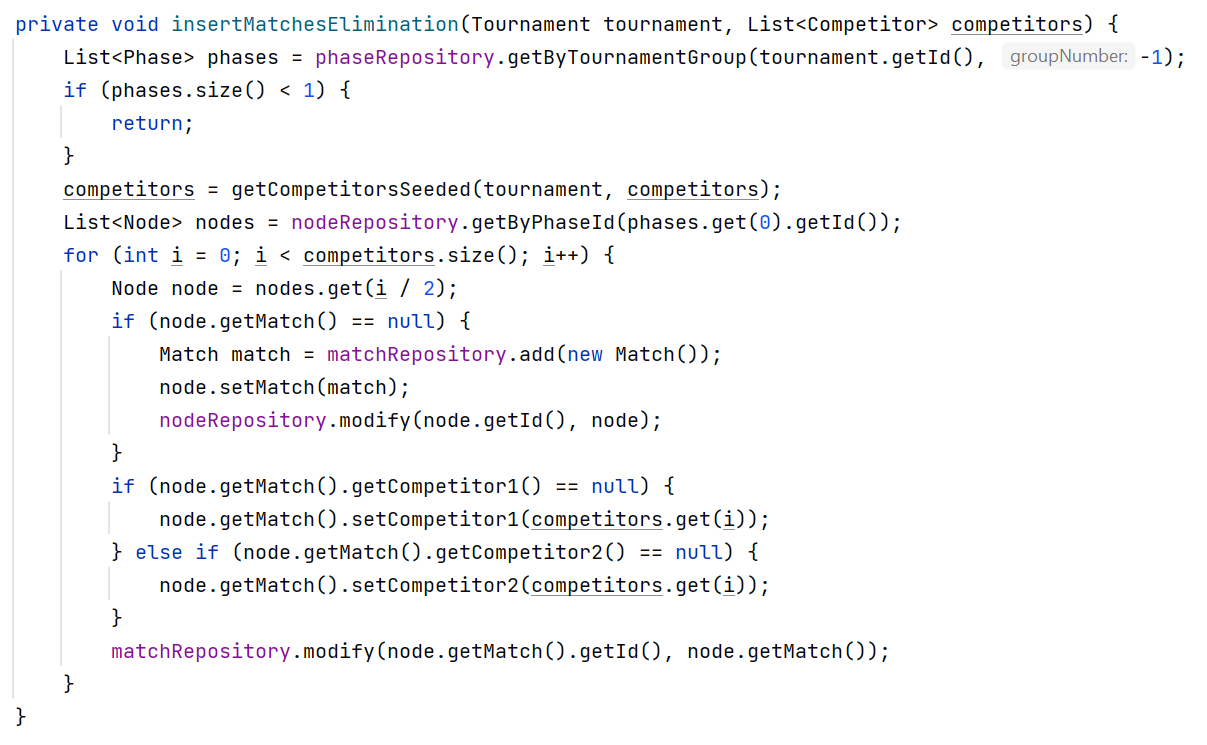
\includegraphics[scale=0.48]{pics/backend/elimination/elimination_insertMatches.png}
    \caption{Einfügen der Matches im Elimination Modus}
\end{figure}

Diese Methode iteriert durch alle Nodes aus der ersten Phase durch, wobei durch "nodes.get(i / 2)" jede Node immer 2 Mal durchlaufen wird. 
Sollte eine Node noch kein Match haben, wird dieses hinzugefügt. Anschließend werden die Teilnehmer/innen, einer pro Durchlauf, also 2 pro Match, 
in die Matches eingefügt. 

\subsubsection{Seeding}

Um Turniere so spannend wie möglich zu gestalten, wird das sogenannte "Seeding" angewendet. Der Seed eines/einer Teilnehmers/in ist eine Einschätzung, wie gut dieser/diese Teilnehmer/in im vergleich zu den anderen im selben Turnier
ist. Somit ist der Seed 1 der/die beste Teilnehmer/in des Turniers, der Seed 2 der/die zweitbeste, usw. Mit Seeding will man erreichen, dass, angenommen der/die Teilnehmer/in mit dem niedrigeren Seed gewinnt immer gegen den/die 
mit dem höheren Seed, die Seeds 1 und 2, also die besten Teilnehmer/innen im Finale gegeneinander antreten. Würde man die Seeds einfach von oben nach unten in das Turnier einfügen, würde folgendes passieren.


\begin{figure}[H]
    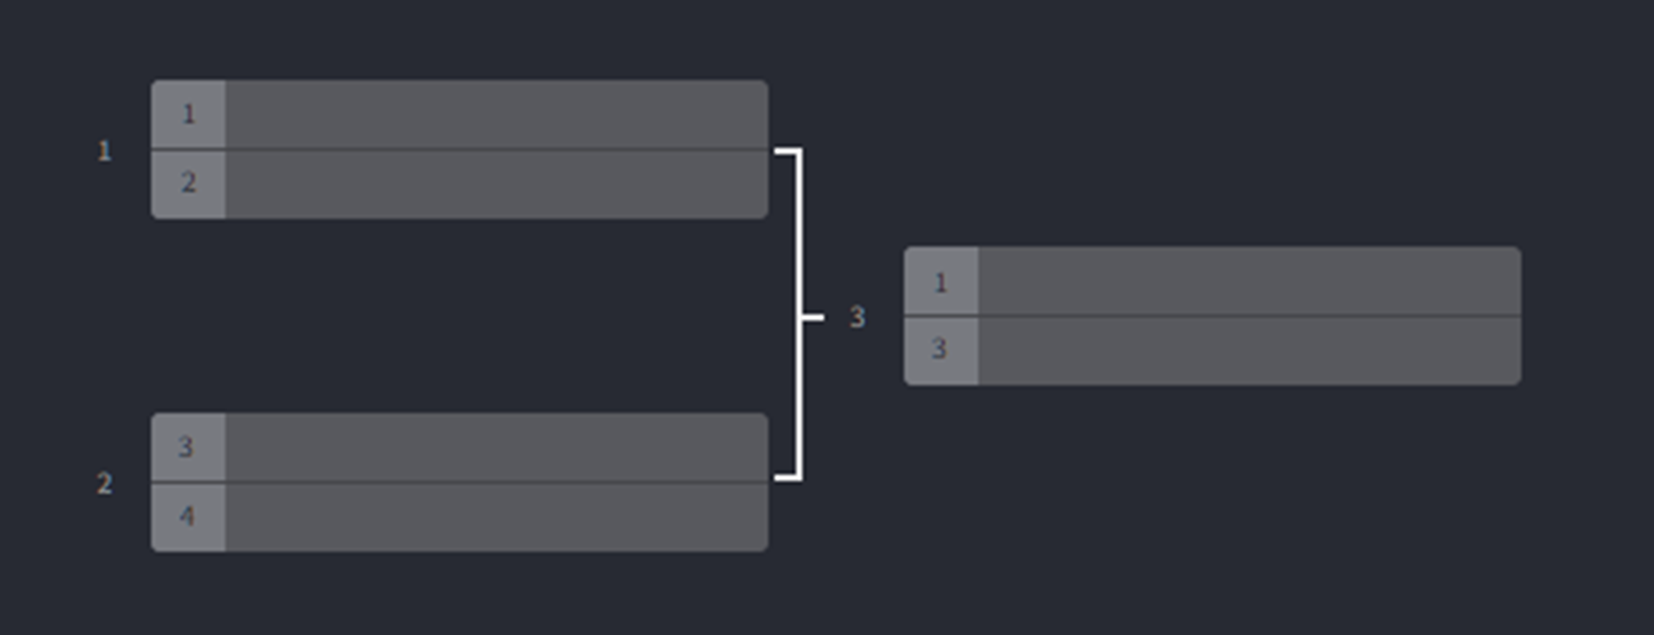
\includegraphics[scale=0.33]{pics/backend/elimination/elimination_tree_seeded_wrong.png}
    \caption{Turnierbaum falsch geseedet\cite{implementation-execution-1}}
\end{figure}

Wie man sieht, treten die ersten beiden Seeds bereits im Halbfinale gegeneinander an, was für ein möglichst spannendes Turnier nicht wirklich wünschenswert ist. Aus diesem Grund werden die Teilnehmer/innen folgendermaßen zusammengeführt.

\begin{figure}[H]
    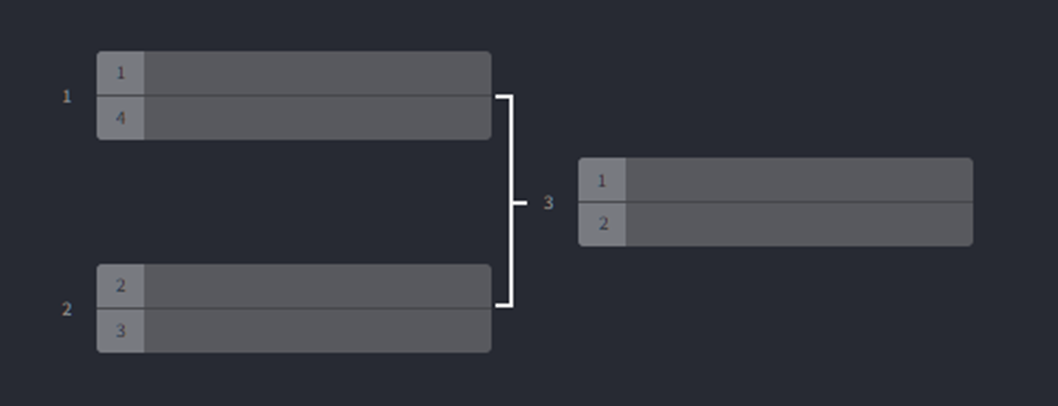
\includegraphics[scale=0.515]{pics/backend/elimination/elimination_tree_seeded.png}
    \caption{Turnierbaum richtig geseedet\cite{implementation-execution-1}}
\end{figure}

Der erste Seed tretet gegen den letzten an, der zweite gegen den vorletzten, usw. Auf diese weise ist es am wahrscheinlichsten, dass das finale Match so spannend wie möglich wird. 
Es steckt jedoch noch ein bisschen mehr dahinter. Sollte man es so machen, dass im ersten Match von oben der erste Seed gegen den letzten antritt, im zweiten von oben der zweite gegen den vorletzten, usw., 
würde bie größeren Turnieren spätestens in der zweiten Phase das selbe Problem nochmal auftreten.

\begin{figure}[H]
    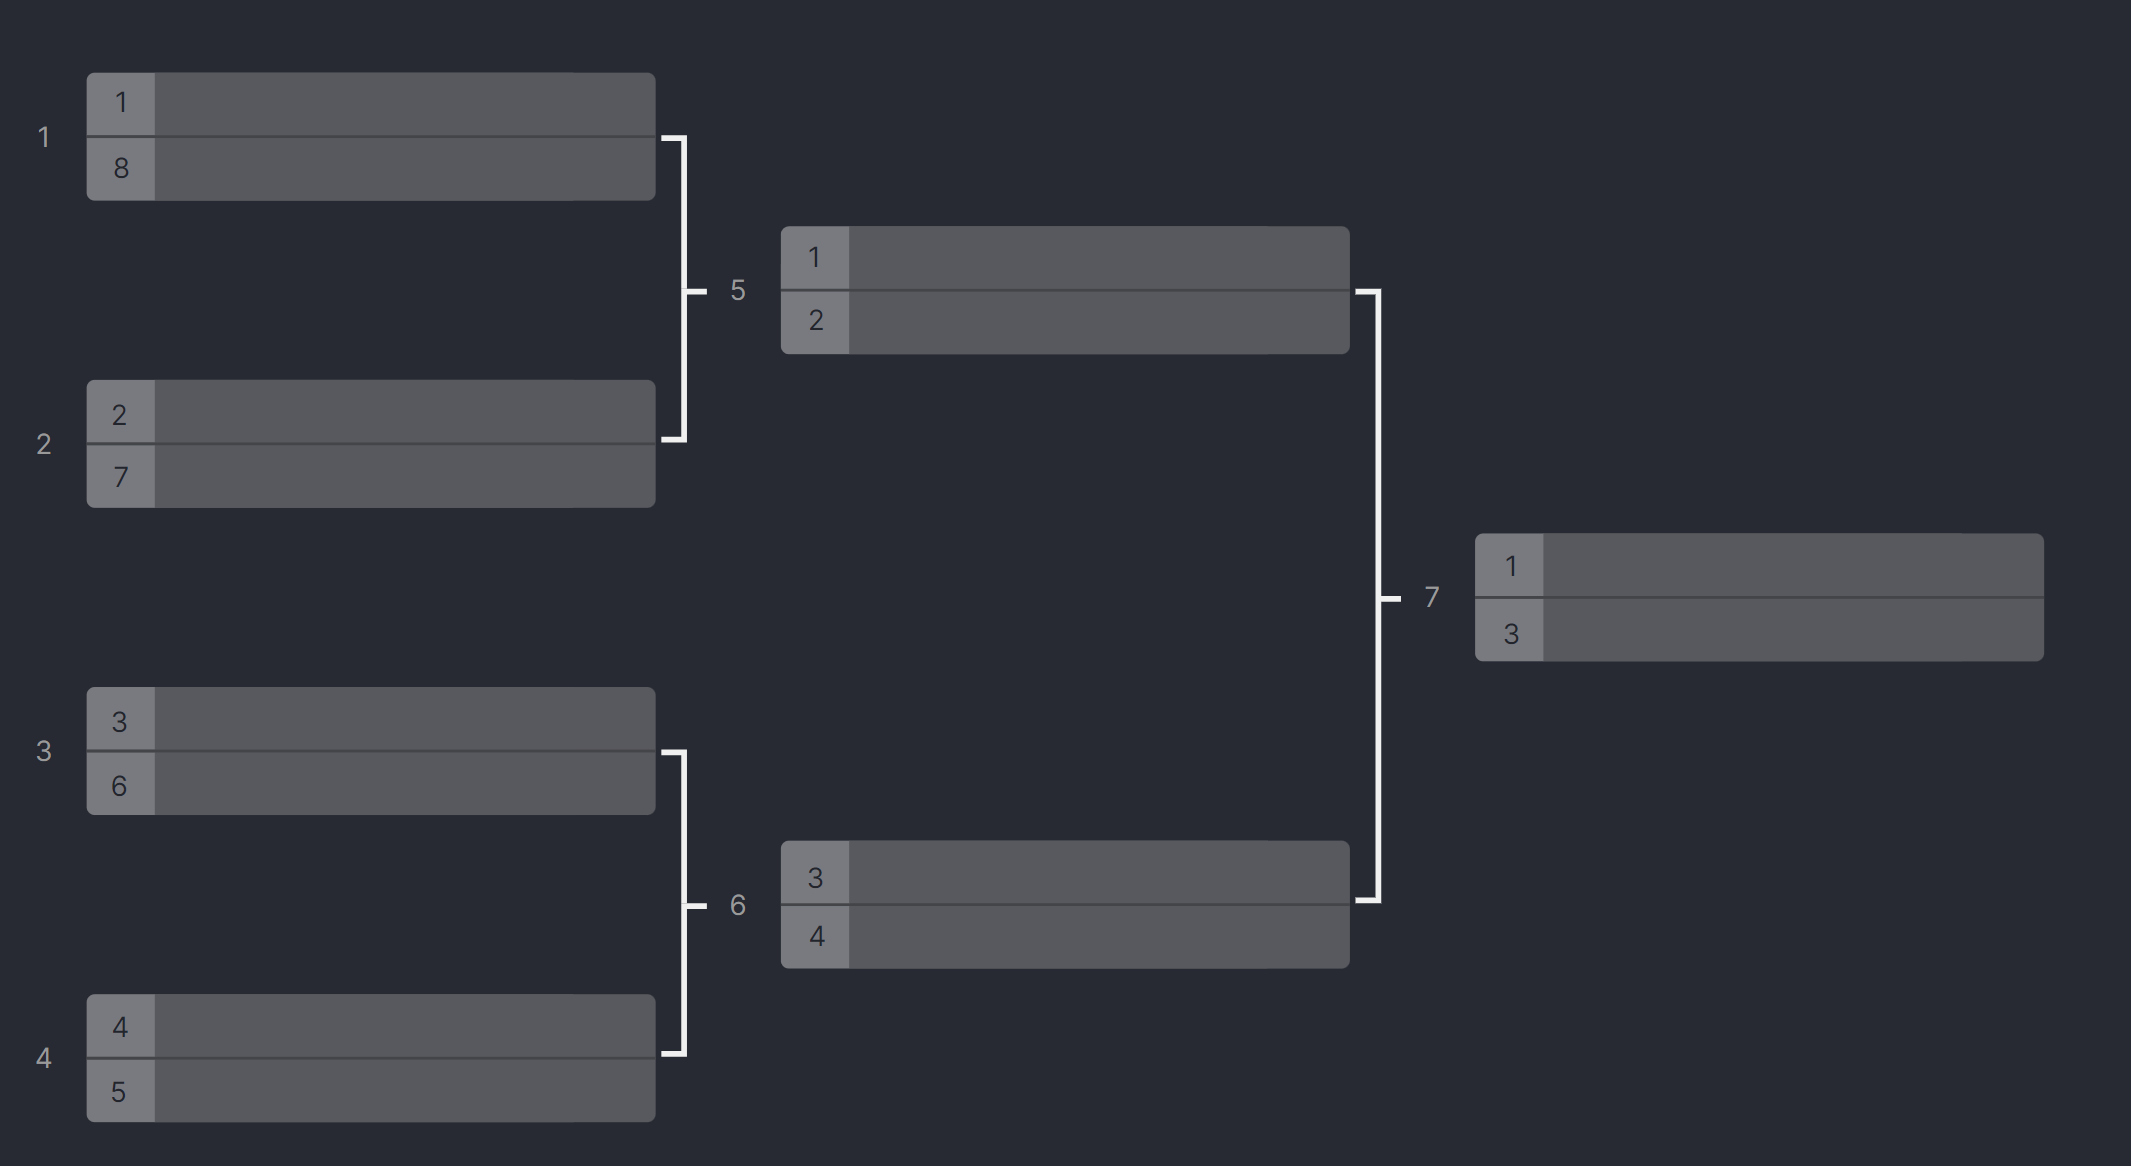
\includegraphics[scale=0.25]{pics/backend/elimination/elimination_tree_seeded_wrong_big.png}
    \caption{großer Turnierbaum falsch geseedet\cite{implementation-execution-1}}
\end{figure}

Um dieses Problem zu beheben, wird beim Anordnen Rekursion verwendet.

\begin{figure}[H]
    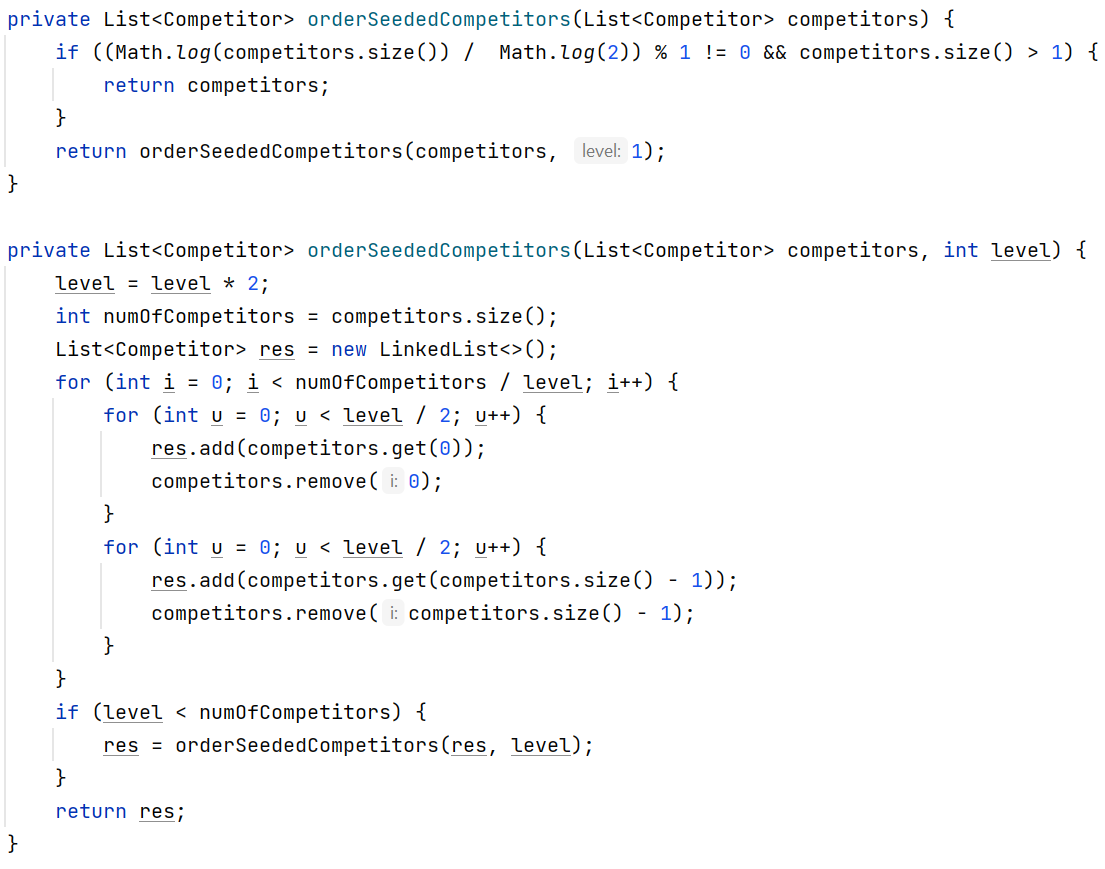
\includegraphics[scale=0.5]{pics/backend/elimination/elimination_orderSeededCompetitors.png}
    \caption{Anordnen der Teilnehmer im Code}
\end{figure}

In der oberen Methode wird geprüft, ob die Anzahl der Teilnehmer/innen eine Hochzahl von 2 ist.
Außerdem wird angenommen, dass die Teilnehmer/innen nach Seed aufsteigend sortiert wurden. Nun wird die untere Methode ausgeführt, 
welche wie schon erwähnt Rekursion beinhaltet. Diese wird mit den folgenden Abbildungen erklärt.

\begin{figure}[H]
    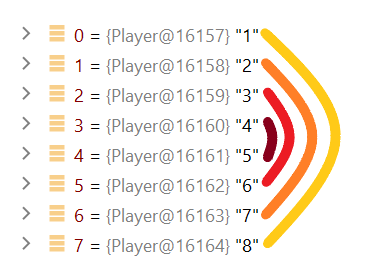
\includegraphics[scale=0.8]{pics/backend/elimination/seeding_1.png}
    \caption{Anordnen der Teilnehmer 1}
    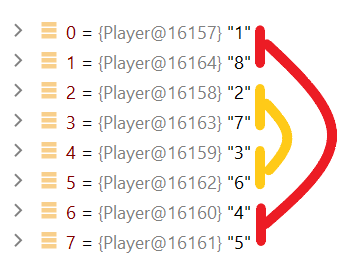
\includegraphics[scale=0.8]{pics/backend/elimination/seeding_2.png}
    \caption{Anordnen der Teilnehmer 2}
    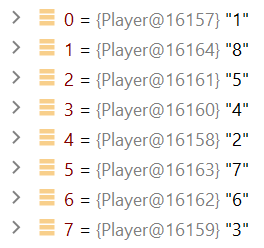
\includegraphics[scale=0.8]{pics/backend/elimination/seeding_3.png}
    \caption{Anordnen der Teilnehmer 3}
\end{figure}

Im Grunde bewirkt dieser Code das gleiche, wie die Lösung von vorhin, nur mehrmals.
Angenommen das Turnier hat 8 Teilnehmer.
Der erste Durchlauf der Methode kümmert sich um die erste Phase, es werden die Seeds 1 und 8 zusammengeführt, 2 und 7, 3 und 6, und 4 und 5.
Der zweite Durchlauf kümmert sich nun um die zweite Phase. In der ersten Phase wird wie erwähnt davon ausgegangen, dass die Seeds 1 bis 4 in die zweite 
Phase aufsteigen, also sollten in der Phase die Seeds 1 und 4, und 2 und 3 zusammengeführt werden.
Dies wird erreicht, indem in der ersten Phase die Seeds 1 und 8 (also in der zweiten Phase nur Seed 1) mit den 
Seeds 4 und 5 (also in der zweiten Phase nur Seed 4) zusammengeführt werden. Das ganze wird so lange wiederholt, bis für jede zukünftige Phase richtig 
angeordnet wurde. Im Turnierbaum sieht es dass so aus.

\begin{figure}[H]
    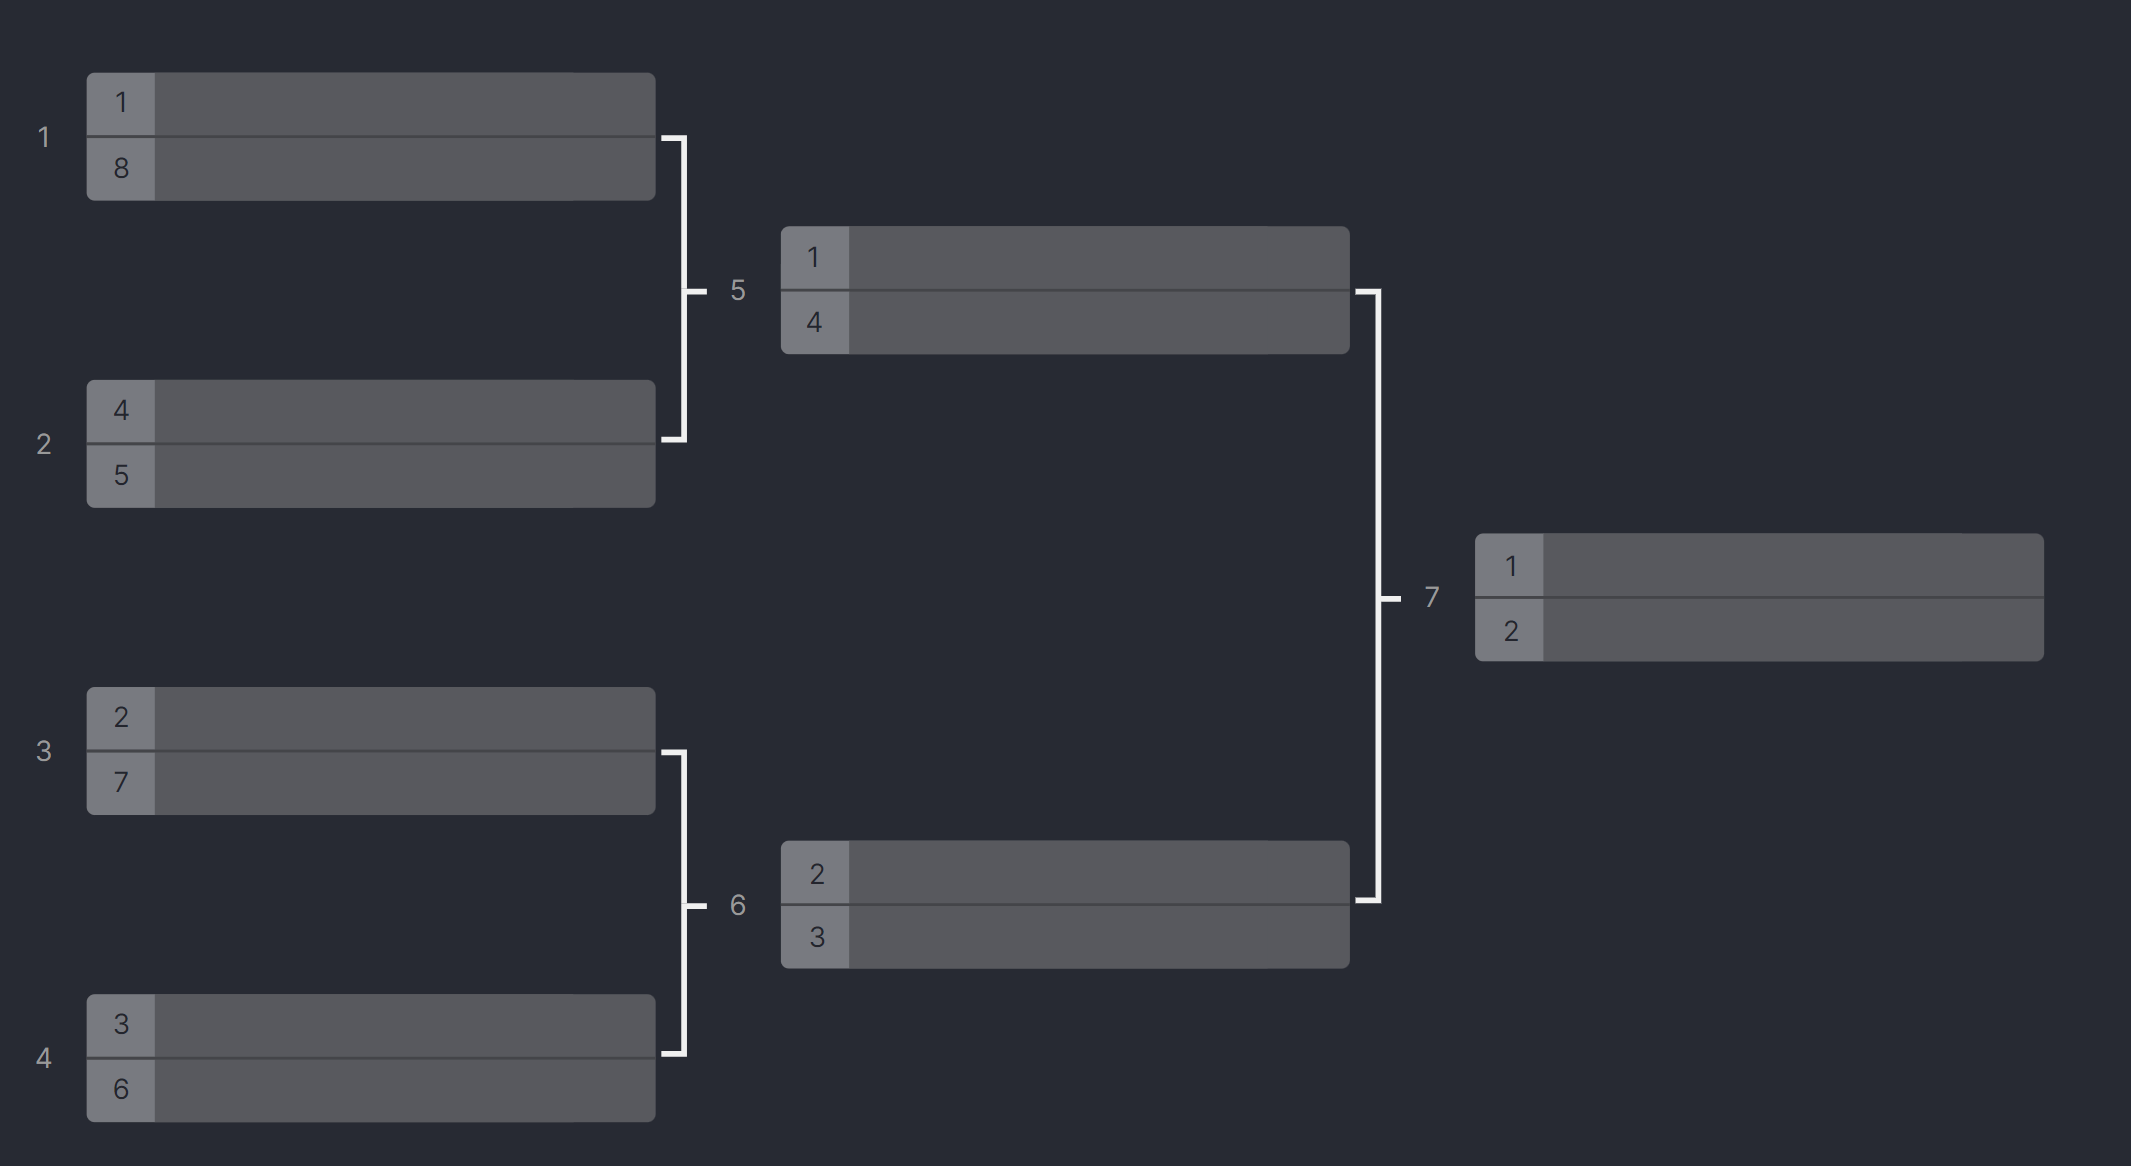
\includegraphics[scale=0.25]{pics/backend/elimination/elimination_tree_seeded_big.png}
    \caption{großer Turnierbaum geseedet\cite{implementation-execution-1}}
\end{figure}

Im Backend gibt es 2 Möglichkeiten, Seeds and Teilnehmer/innen zu verteilen. Die erste Möglichkeit ist es, die Teilnehmer nach der durchnittlichen Plazierung aus vergangenen Turnieren zu sortieren, 
jedoch setzt das voraus, dass die Teilnehmer schon an Turniern teilgenommen haben. Sollte dies nicht der Fall sein, ist die zweite Möglichkeit, dass die Teilnehmer manuell vom Turnierorganisator sortiert werden.
Hier ist es allerdings von großer bedeutung, einen vertrauenswürdigen Turnierorganisator haben, denn, wie man oben sieht, je besser man im Vergleich zu anderen Teilnehmern eingeschätzt wird, desto leichtere Gegner wird man bekommen.

\subsubsection{Buy-Rounds}

Sollte die Anzahl der Teilnehmer/innen in einem Turnier keine Hochzahl von 2 sein, ist es nicht möglich, in der ersten Phase jedem/jeder Teilnehmer/in einen Gegner zu geben. 
Um dieses Problem zu lösen, steigen manche Teilnehmer automatisch in die zweite Phase auf, ohne ein Match gewonnen zu haben.

\begin{figure}[H]
    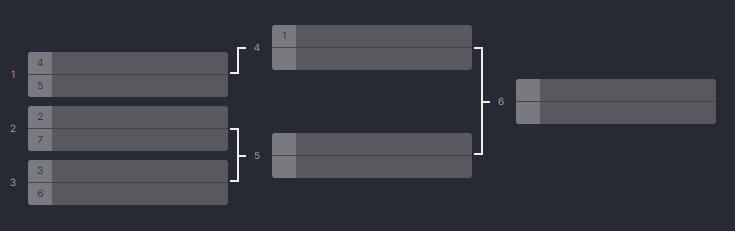
\includegraphics[scale=0.75]{pics/backend/elimination/elimination_buy_rounds.png}
    \caption{Turnierbaum mit Buy-Rounds\cite{implementation-execution-1}}
\end{figure}

Im Code wird das mit diesen Methoden erreicht.

\begin{figure}[H]
    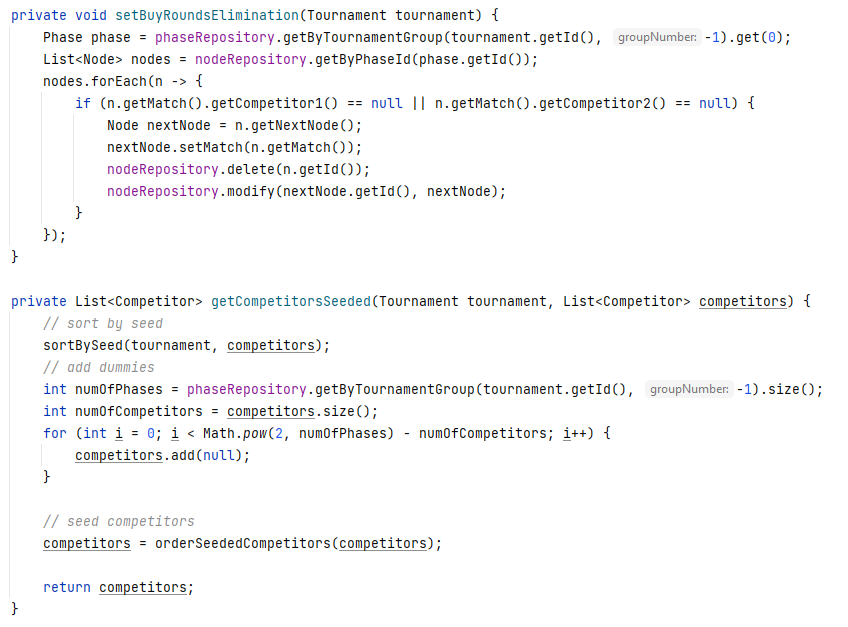
\includegraphics[scale=0.65]{pics/backend/elimination/elimination_setBuyRounds.png}
    \caption{Buy-Rounds im Elimination Modus}
\end{figure}

Die untere Methode gibt alle Teilnehmer/innen des Turniers zurück, und zwar bereits nach Seed angeordnet. Besonders wichtig ist für Buy-Rounds der mittlere Teil der Methode. Angenommen ein Turnier hat 5 Teilnehmer/innen. 
Die nächste Hochzahl wäre in dem Fall 8, also befüllt diese Methode die Teilnehmerliste mit 3 "dummy" Teilnehmern, sodass die Teilnehmeranzahl eine Hochzahl von 2 ist. Dies ist notwendig, um die Teilnehmer/innen korrekt 
nach Seed anzuordnen. 

Nun sind jedoch 3 "dummy" Teilnehmer in der Teilnehmerliste, mit denen man nichts anfangen kann. Um diese kümmert sich nun die obere Methode. Jeder/jede Teilnehmer/in, der einen "dummy" Teilnehmer als Gegner hat, 
steigt automatisch in die zweite Phase auf, und spielt dort das erste Match.

\subsection{Round Robin}

Im Round Robin Turniermodus tritt jeder/jede Teilnehmer/in gegen jeden Teilnehmer an, egal, wie oft man gewinnt oder verliert. Somit entsteht hier kein Turnierbaum, sondern eher ein Turnierraster aus Matches.

\begin{figure}[H]
    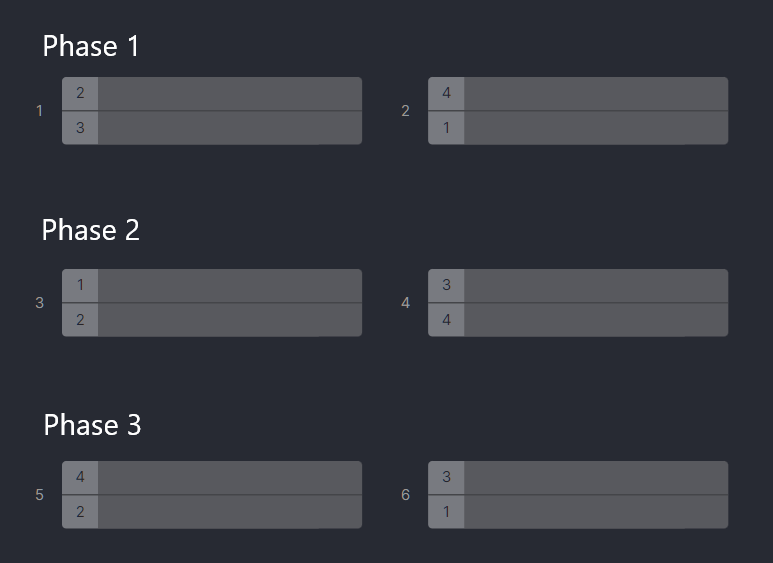
\includegraphics[scale=0.5]{pics/backend/roundrobin/roundrobin_grid.png}
    \caption{Turnierraster\cite{implementation-execution-1}}
\end{figure}

\subsubsection{Phases}

Die Phasenanzahl im Round Robin Turniermodus ist etwas einfacher zu errechnen, als bei Elimination. Angenommen ein Turnier hat 4 Teilnehmer/innen, somit hat jeder/jede Teilnehmer/in insgesammt 3 Gegner. Da jeder/jede Teilnehmer/in in jeder Phase 
ein Match spielen kann, gibt es hier 3 Phasen, also die Teilnehmeranzahl - 1. Bei einer ungeraden Teilnehmeranzahl ist es jedoch etwas anders, da in jeder Phase ein/eine Teilnehmer keinen Gegner hat. Daher wäre hier die Phasenanzahl gleich 
der Teilnehmeranzahl.

\begin{figure}[H]
    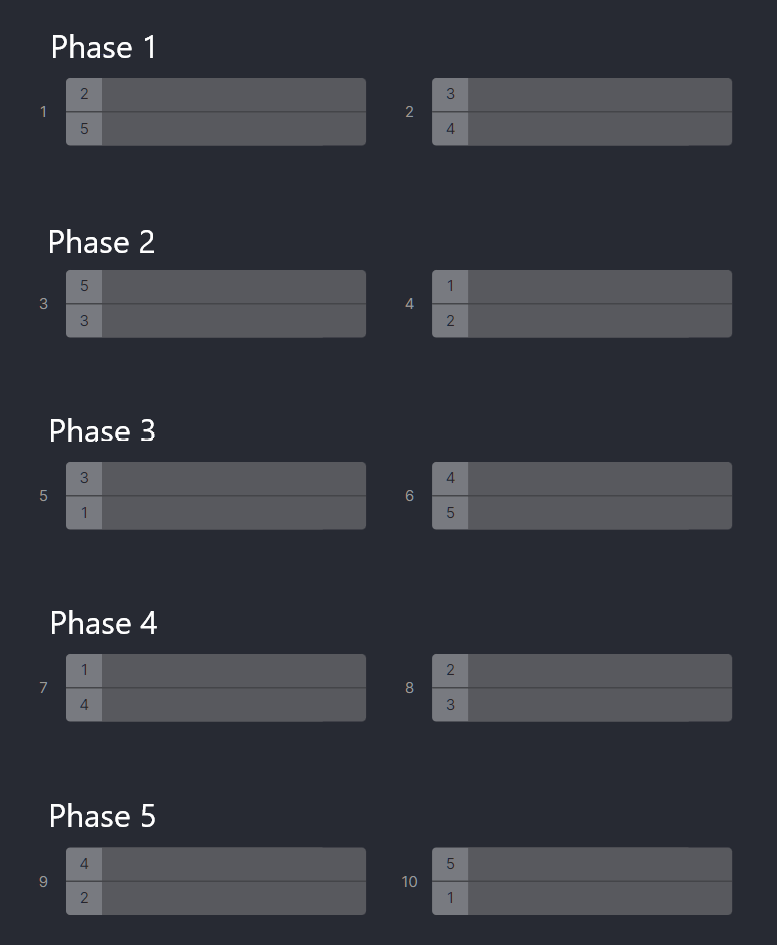
\includegraphics[scale=0.5]{pics/backend/roundrobin/roundrobin_grid_uneven.png}
    \caption{Turnierraster mit ungerader Teilnehmeranzahl\cite{implementation-execution-1}}
\end{figure}

Die Rechnung im Code sieht folgendermaßen aus.

\begin{figure}[H]
    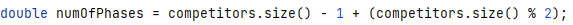
\includegraphics[scale=1]{pics/backend/roundrobin/roundrobin_insertPhases.png}
    \caption{Einfügen der Phasen im Round Robin Modus}
\end{figure}

\subsubsection{Nodes und Matches}

Da im Round Robin Turniermodus schon im Vorhinein bekannt ist, wer wann gegen wen antritt, werden hier Nodes und Matches gleichzeitig eingefügt. Dafür ist diese Methode verantwortlich.

\begin{figure}[H]
    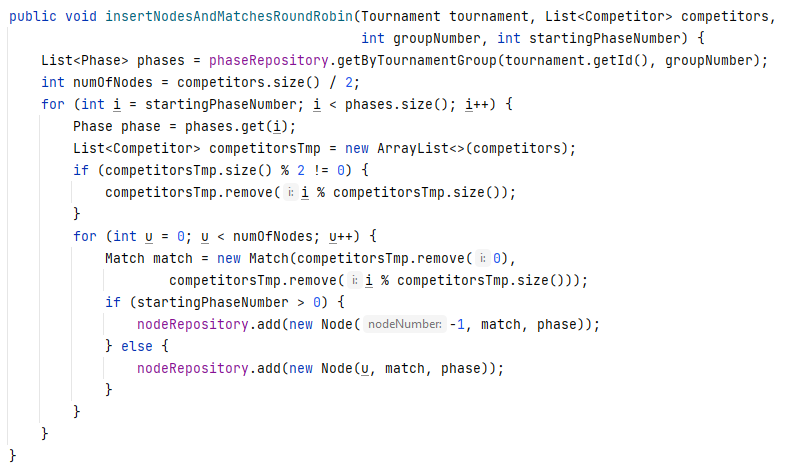
\includegraphics[scale=0.7]{pics/backend/roundrobin/roundrobin_insertNodesAndMatches.png}
    \caption{Einfügen der Nodes und Matches im Round Robin Modus}
\end{figure}

Ein/eine Teilnehmer/in muss in jeder Phase gegen verschiedene Teilnehmer/innen antreten. In der ersten Phase nimmt die Methode aus der Teilnehmerliste den/die erste/n Teilnehmer/in, und den/die unmittelbar danach, und fügt sie zusammen, 
so lange, bis keine Teilnehmer/innen mehr in der Liste sind.

\begin{figure}[H]
    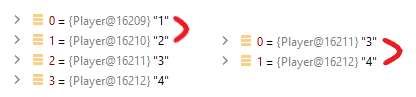
\includegraphics[scale=0.8]{pics/backend/roundrobin/matching_up_1.png}
    \caption{Round Robin Algorithmus 1}
\end{figure}